\section{Background}\label{sec:background}

\subsection{PFC Deadlock Problem}\label{subsec:pfcdeadlock}

The deployment of RDMA over Ethernet requires Priority-based Flow Control (PFC)~\cite{pfc}  to provide a lossless L2 network~\cite{dcqcn, rdmaatscale}. 
PFC is a mechanism for ensuring zero packet loss under congestion in data center bridging (DCB) networks. When PFC is enabled, the switch will maintain a counter to track the virtual queue length of each ingress queue. Once the queue length reaches a pre-configured PFC threshold, a PAUSE frame will be generated to pause the incoming link for a specified period of time.

The using of PFC will cause PFC deadlock problem, as reported in ~\cite{rdmaatscale}. PFC deadlock arises when the buffer usage of a set of ingress queues reach their PFC thresholds simultaneously, and the paused links form a cycle. Once PFC deadlock is created, no packet is allowed to be transmitted through the affected links. 

Due to the backpressue paradigm of PFC~\cite{tcp-bolt,dcqcn}, data transmission of the whole DCN may be paused by a PFC deadlock only among a small number of network devices. Hence it is important to avoid PFC deadlock in DCN.



\subsection{Cyclic Buffer Dependency}\label{subsec:cyclicbd}

Cyclic buffer dependency is a well-known necessary condition for deadlock problem~\cite{gerla1980flow,dally}.

For a given DCN topology $\textbf{N}$ and a routing function $\textbf{R}$, we can construct the corresponding buffer dependency graph as follows. For any two ingress queues $RX_1$ and $RX_2$ in $\textbf{N}$, if there exists a path $p$ that traverses $RX_1$ and  $RX_2$ consecutively, we add a directed dependency edge from $RX_1$ to $RX_2$.  If there are cycles in the constructed buffer dependency graph, we say ($\textbf{N}$, $\textbf{R}$) has cyclic buffer dependency. PFC deadlock could occur when there is cyclic buffer dependency.

PFC deadlock can be avoided by adopting a deadlock-free routing function $\textbf{R}$ that will not create cyclic buffer dependency. Many algorithms have been proposed in the past for producing deadlock-free routing functions for a given network topology~\cite{dally,flich2012survey,tcp-bolt}.

%\subsection{Classification of PFC Deadlock}\label{subsec:deadlockclassification}
%
%PFC Deadlock can be classified into 

\subsection{Deadlock Time in High-speed Network}\label{subsec:deadlocktime}

\begin{figure}[t]
	\centering
	\subfloat[short for lof][Topology and flows.]{
		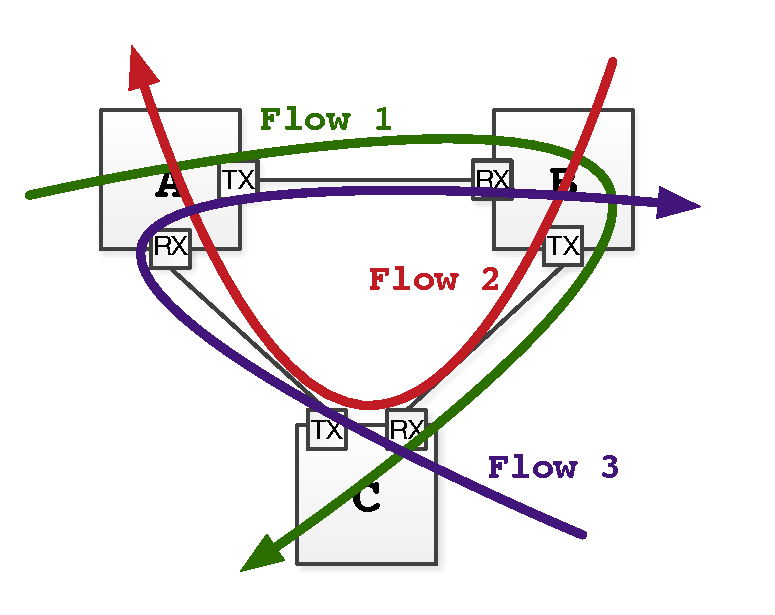
\includegraphics[width=0.27\textwidth] {figs/deadlock_time_a}
	}
	\subfloat[short for lof][Buffer dependency graph.]{
		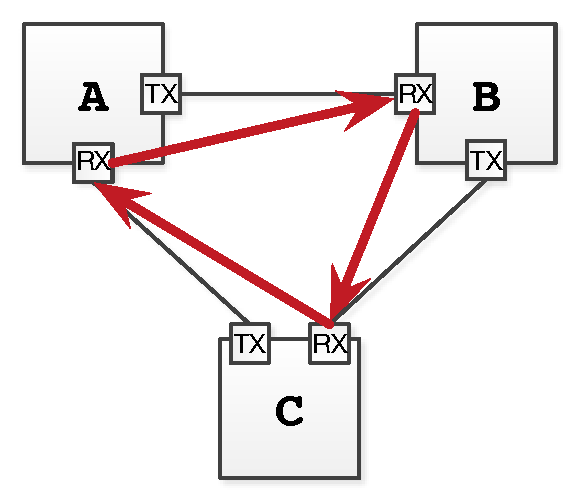
\includegraphics[width=0.22\textwidth] {figs/deadlock_time_b}
	}
	
		\subfloat[short for lof][Time to create a PFC deadlock.]{
			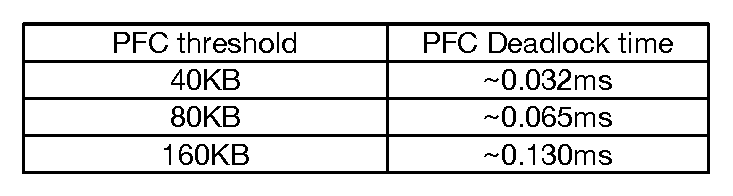
\includegraphics[width=0.45\textwidth] {figs/deadlock_time_c}
		}
	\caption{Measurement of the time to create a PFC deadlock in a 3-switch network.}\label{fig:deadlocktime}
	\vspace{-0.2in}
\end{figure}

Switches deployed in current DCNs are shallow-buffered commodity switches with only about 8-12MB buffer. As the link capacity goes up to 40Gbps or even more,  switch buffer can be consumed in just a few milliseconds under congestion. This fact also indicates that once cyclic buffer dependency is met, deadlock can occur within a very short time.

We did a packet-level NS-3 simulation to measure how long it will take to create a PFC deadlock. We choose simulation instead of real testbed experiment because we need a well-controlled environment for conducting accurate measurement. 
As shown In Fig.~\ref{fig:deadlocktime}(a), our simulation is performed ina 3-switch network. The link capacity is 40Gbps, and each switch has 12MB buffer. We inject three UDP fows with infinite traffic demand into the network simultaneously. The paths taken by these flows form a cyclic buffer dependency as shown in Fig.~\ref{fig:deadlocktime}(b).

As shown in Fig.~\ref{fig:deadlocktime}(c), PFC deadlock occurs in less than 0.2ms when setting various PFC thresholds. Note that 160KB is already a sufficiently large PFC threshold in practice~\cite{dcqcn}. The results indicate that once we have cyclic buffer dependency in the network, PFC deadlock can occur in a very short time under 40Gbps DCNs.
